\documentclass{article}

% Packages required by doxygen
\usepackage{calc}
\usepackage{doxygen}
\usepackage{graphicx}
\usepackage[utf8]{inputenc}
\usepackage{makeidx}
\usepackage{multicol}
\usepackage{multirow}
\usepackage{textcomp}
\usepackage[table]{xcolor}

% NLS support packages
\usepackage{polski}
\usepackage[T1]{fontenc}

% Font selection
\usepackage[T1]{fontenc}
\usepackage{mathptmx}
\usepackage[scaled=.90]{helvet}
\usepackage{courier}
\usepackage{amssymb}
\usepackage{sectsty}
\renewcommand{\familydefault}{\sfdefault}
\allsectionsfont{%
  \fontseries{bc}\selectfont%
  \color{darkgray}%
}
\renewcommand{\DoxyLabelFont}{%
  \fontseries{bc}\selectfont%
  \color{darkgray}%
}

% Page & text layout
\usepackage{geometry}
\geometry{%
  a4paper,%
  top=2.5cm,%
  bottom=2.5cm,%
  left=2.5cm,%
  right=2.5cm%
}
\tolerance=750
\hfuzz=15pt
\hbadness=750
\setlength{\emergencystretch}{15pt}
\setlength{\parindent}{0cm}
\setlength{\parskip}{0.2cm}
\makeatletter
\renewcommand{\paragraph}{%
  \@startsection{paragraph}{4}{0ex}{-1.0ex}{1.0ex}{%
    \normalfont\normalsize\bfseries\SS@parafont%
  }%
}
\renewcommand{\subparagraph}{%
  \@startsection{subparagraph}{5}{0ex}{-1.0ex}{1.0ex}{%
    \normalfont\normalsize\bfseries\SS@subparafont%
  }%
}
\makeatother

% Headers & footers
\usepackage{fancyhdr}
\pagestyle{fancyplain}
\fancyhead[LE]{\fancyplain{}{\bfseries\thepage}}
\fancyhead[CE]{\fancyplain{}{}}
\fancyhead[RE]{\fancyplain{}{\bfseries\leftmark}}
\fancyhead[LO]{\fancyplain{}{\bfseries\rightmark}}
\fancyhead[CO]{\fancyplain{}{}}
\fancyhead[RO]{\fancyplain{}{\bfseries\thepage}}
\fancyfoot[LE]{\fancyplain{}{}}
\fancyfoot[CE]{\fancyplain{}{}}
\fancyfoot[RE]{\fancyplain{}{\bfseries\scriptsize Wygenerowano N, 15 mar 2015 20\-:19\-:16 dla Lab01 -\/ mnożenie przez 2 programem Doxygen }}
\fancyfoot[LO]{\fancyplain{}{\bfseries\scriptsize Wygenerowano N, 15 mar 2015 20\-:19\-:16 dla Lab01 -\/ mnożenie przez 2 programem Doxygen }}
\fancyfoot[CO]{\fancyplain{}{}}
\fancyfoot[RO]{\fancyplain{}{}}
\renewcommand{\footrulewidth}{0.4pt}
\renewcommand{\chaptermark}[1]{%
  \markboth{#1}{}%
}
\renewcommand{\sectionmark}[1]{%
  \markright{\thesection\ #1}%
}

% Indices & bibliography
\usepackage{natbib}
\usepackage[titles]{tocloft}
\setcounter{tocdepth}{3}
\setcounter{secnumdepth}{5}
\makeindex

% Hyperlinks (required, but should be loaded last)
\usepackage{ifpdf}
\ifpdf
  \usepackage[pdftex,pagebackref=true]{hyperref}
\else
  \usepackage[ps2pdf,pagebackref=true]{hyperref}
\fi
\hypersetup{%
  colorlinks=true,%
  linkcolor=blue,%
  citecolor=blue,%
  unicode%
}

% Custom commands
\newcommand{\clearemptydoublepage}{%
  \newpage{\pagestyle{empty}\cleardoublepage}%
}


%===== C O N T E N T S =====

\begin{document}

% Titlepage & ToC
\hypersetup{pageanchor=false}
\pagenumbering{roman}
\begin{titlepage}
\vspace*{7cm}
\begin{center}%
{\Large Lab01 -\/ mnożenie przez 2 }\\
\vspace*{1cm}
{\large Mateusz Krawczuk, nr indeksu 209147}\\
\vspace{0.5cm}
{\large Wygenerowano przez Doxygen 1.8.6}\\
\vspace*{0.5cm}
{\small N, 15 mar 2015 20:19:16}\\
\end{center}
\end{titlepage}
%\clearemptydoublepage
%\tableofcontents
%\clearemptydoublepage
\pagenumbering{arabic}
%\hypersetup{pageanchor=true}

%--- Begin generated contents ---
\part{Streszczenie}
Niniejszy dokument zawiera wyniki pomiaru czasu, którego potrzebował mój komputer na wykonanie operacji mnożenia przez 2 na zestawach danych o długościach od 1 do 10e8 elementów. Zawiera także dokumentację kodu programu użytego do wykonania tego badania.

\part{Sprawozdanie}
Obliczenia wykonano na 64-bitowym procesorze AMD Athlon X2. Wykres przedstawia zależność czasu wykonywania operacji od długości ciągu danych. Został wygenerowany za pomocą Gnuplota. Podziałki na obydwu osiach są w skali logarytmicznej. Na wykresie umieszczono także prostą y = (0.7803/10e8)x. Dzięki temu lepiej widać, że jest to zależność mocno zbliżona do liniowej - można na tej podstawie domniemywać, że złożoność obliczeniowa tej operacji jest O(n). Warto zwrócić uwagę na długość wykonywania operacji na jednym elemencie danych - przewyższa on o rząd wielkości czas wykonywania na dziesięciu elementach.
\centerline{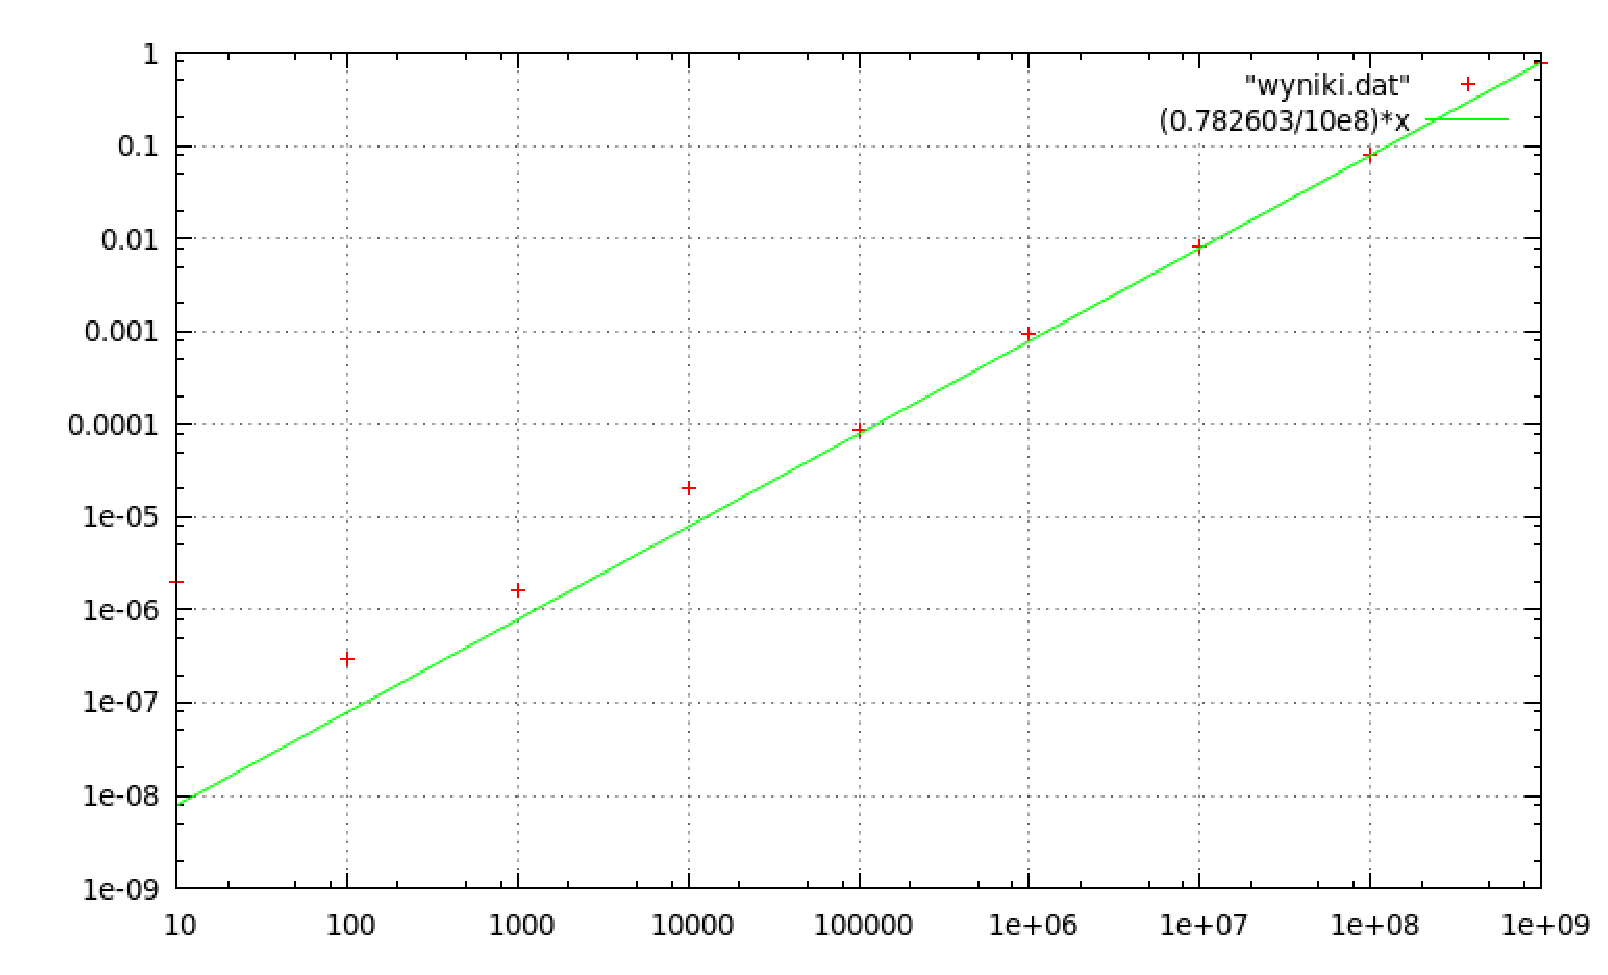
\includegraphics[width=\textwidth,height=\textheight,keepaspectratio]{wykres1.eps}}

\part{Dokumentacja kodu}
\hypertarget{benchmark_8h}{\section{Dokumentacja pliku benchmark.\-h}
\label{benchmark_8h}\index{benchmark.\-h@{benchmark.\-h}}
}


Deklaracje funkcji związanych z analizą prędkości operacji.  


{\ttfamily \#include \char`\"{}operacja.\-h\char`\"{}}\\*
{\ttfamily \#include \char`\"{}ustawienia.\-h\char`\"{}}\\*
{\ttfamily \#include \char`\"{}kontener.\-h\char`\"{}}\\*
{\ttfamily \#include \char`\"{}stos.\-h\char`\"{}}\\*
{\ttfamily \#include \char`\"{}kolejka.\-h\char`\"{}}\\*
{\ttfamily \#include \char`\"{}stos\-\_\-arr.\-h\char`\"{}}\\*
{\ttfamily \#include $<$fstream$>$}\\*
{\ttfamily \#include $<$iostream$>$}\\*
{\ttfamily \#include $<$vector$>$}\\*
{\ttfamily \#include $<$cstdlib$>$}\\*
{\ttfamily \#include $<$cmath$>$}\\*
\subsection*{Funkcje}
\begin{DoxyCompactItemize}
\item 
void \hyperlink{benchmark_8h_aa64f5c659f0dd5f25435b15c1e1fa7f5}{Benchmark} ()
\begin{DoxyCompactList}\small\item\em Główna funkcja programu. \end{DoxyCompactList}\item 
int \hyperlink{benchmark_8h_a43bc241c88791024a92dc76ff18d0d48}{licz\-\_\-dekady} (int dlugosc\-\_\-ciagu)
\begin{DoxyCompactList}\small\item\em Funkcja pomocnicza do określania ilości dekad. \end{DoxyCompactList}\end{DoxyCompactItemize}


\subsection{Opis szczegółowy}
Plik zawiera deklaracje funkcji \hyperlink{benchmark_8h_aa64f5c659f0dd5f25435b15c1e1fa7f5}{Benchmark()} oraz \hyperlink{benchmark_8h_a43bc241c88791024a92dc76ff18d0d48}{licz\-\_\-dekady()}. Funkcja \hyperlink{benchmark_8h_aa64f5c659f0dd5f25435b15c1e1fa7f5}{Benchmark()} jest główną funkcją programu benchmarkującego, natomiast funkcja \hyperlink{benchmark_8h_a43bc241c88791024a92dc76ff18d0d48}{licz\-\_\-dekady()} jest funkcją pomocniczą wywoływaną w funkcji \hyperlink{benchmark_8h_aa64f5c659f0dd5f25435b15c1e1fa7f5}{Benchmark()}. 

Definicja w pliku \hyperlink{benchmark_8h_source}{benchmark.\-h}.



\subsection{Dokumentacja funkcji}
\hypertarget{benchmark_8h_aa64f5c659f0dd5f25435b15c1e1fa7f5}{\index{benchmark.\-h@{benchmark.\-h}!Benchmark@{Benchmark}}
\index{Benchmark@{Benchmark}!benchmark.h@{benchmark.\-h}}
\subsubsection[{Benchmark}]{\setlength{\rightskip}{0pt plus 5cm}void Benchmark (
\begin{DoxyParamCaption}
{}
\end{DoxyParamCaption}
)}}\label{benchmark_8h_aa64f5c659f0dd5f25435b15c1e1fa7f5}
Funkcja wywoływana w funkcji \hyperlink{main_8cpp_ae66f6b31b5ad750f1fe042a706a4e3d4}{main()}. Nie przyjmuje argumentów ani nie zwraca wartości. Funkcja otwiera plik, który powinien zawierać ciąg danych, na których przeprowadzona zostanie operacja. Otwiera także plik, do którego zapisane mają zostać wyniki czasowe operacji. Nazwy plików określone są w nagłówku \char`\"{}ustawienia.\-h\char`\"{}. Z pliku wejściowego wczytuje do obiektu klasy std\-::vector ciąg danych. Do zmiennej typu clock\-\_\-t zostaje zapisany czas procesora od rozpoczęcia procesu. Do funkcji \hyperlink{operacja_8h_a7de44f86b01513b6593ff27e0f62645e}{operacja()} zostaje przekazana referencja do obiektu zawierającego ciąg danych. Po wyjściu z funkcji \hyperlink{operacja_8h_a7de44f86b01513b6593ff27e0f62645e}{operacja()} do zmiennej typu clock\-\_\-t() zostaje tym razem zapisana różnica czasów procesora pomiędzy rozpoczęciem procesu a wartością typu clock\-\_\-t zwróconą przez funkcję \hyperlink{operacja_8h_a7de44f86b01513b6593ff27e0f62645e}{operacja()}. Czas ten przeliczany jest na sekundy i zapisany do pliku wyjściowego. W \char`\"{}ustawienia.\-h\char`\"{} określona jest ilość powtórzeń pomiaru. Pomiary zaczynają się od operacji na jednej wartości i kończą na ciąu danych o długości największej potęgi dziesiątki. Pomiary powtarzane są co dekadę. Informację o największej potędze dziesiątki dostarcza funkcja \hyperlink{benchmark_8h_a43bc241c88791024a92dc76ff18d0d48}{licz\-\_\-dekady()}. 

Definicja w linii 4 pliku benchmark.\-cpp.

\hypertarget{benchmark_8h_a43bc241c88791024a92dc76ff18d0d48}{\index{benchmark.\-h@{benchmark.\-h}!licz\-\_\-dekady@{licz\-\_\-dekady}}
\index{licz\-\_\-dekady@{licz\-\_\-dekady}!benchmark.h@{benchmark.\-h}}
\subsubsection[{licz\-\_\-dekady}]{\setlength{\rightskip}{0pt plus 5cm}int licz\-\_\-dekady (
\begin{DoxyParamCaption}
\item[{int}]{dlugosc\-\_\-ciagu}
\end{DoxyParamCaption}
)}}\label{benchmark_8h_a43bc241c88791024a92dc76ff18d0d48}
Przyjmuje jako argument liczbę całkowitą reprezentującą długość ciągu danych i zaokrągla ją w dół do najbliższej potęgi liczby 10.


\begin{DoxyParams}[1]{Parametry}
\mbox{\tt in}  & {\em dlugosc\-\_\-ciagu} & Długość ciągu danych. \\
\hline
\end{DoxyParams}
\begin{DoxyReturn}{Zwraca}
Zwraca zaokrąglenie w dół do najbliższej potęgi dziesiątki wartości dlugosc\-\_\-ciagu. 
\end{DoxyReturn}


Definicja w linii 59 pliku benchmark.\-cpp.


\hypertarget{operacja_8h}{\section{Dokumentacja pliku operacja.\-h}
\label{operacja_8h}\index{operacja.\-h@{operacja.\-h}}
}


Plik zawiera deklarację funkcji \hyperlink{operacja_8h_ac4193d25d93c09e2404bdb7c7a27334a}{operacja()}.  


{\ttfamily \#include $<$vector$>$}\\*
{\ttfamily \#include $<$cassert$>$}\\*
\subsection*{Funkcje}
\begin{DoxyCompactItemize}
\item 
void \hyperlink{operacja_8h_ac4193d25d93c09e2404bdb7c7a27334a}{operacja} (std\-::vector$<$ int $>$ \&wektor, unsigned int ilosc\-\_\-operacji)
\begin{DoxyCompactList}\small\item\em Wykonuje operację na wczytanym ciągu danych. \end{DoxyCompactList}\end{DoxyCompactItemize}


\subsection{Dokumentacja funkcji}
\hypertarget{operacja_8h_ac4193d25d93c09e2404bdb7c7a27334a}{\index{operacja.\-h@{operacja.\-h}!operacja@{operacja}}
\index{operacja@{operacja}!operacja.h@{operacja.\-h}}
\subsubsection[{operacja}]{\setlength{\rightskip}{0pt plus 5cm}void operacja (
\begin{DoxyParamCaption}
\item[{std\-::vector$<$ int $>$ \&}]{wektor, }
\item[{unsigned int}]{ilosc\-\_\-operacji}
\end{DoxyParamCaption}
)}}\label{operacja_8h_ac4193d25d93c09e2404bdb7c7a27334a}
Funkcja odpowiada za wykonanie porządanej operacji na ciągu danych.


\begin{DoxyParams}[1]{Parametry}
\mbox{\tt in}  & {\em wektor} & Referencja do wczytanego ciąg danych. \\
\hline
\mbox{\tt in}  & {\em ilosc\-\_\-operacji} & Określa na ilu pierwszych elementach wektora wektor ma zostać wykonana operacja. \\
\hline
\end{DoxyParams}


Definicja w linii 10 pliku operacja.\-cpp.


\hypertarget{ustawienia_8h}{\section{Dokumentacja pliku ustawienia.\-h}
\label{ustawienia_8h}\index{ustawienia.\-h@{ustawienia.\-h}}
}


Plik zawiera stałe preprocesora związane z generowaniem, obróbką i pomiarem właściwości danych.  


\subsection*{Definicje}
\begin{DoxyCompactItemize}
\item 
\#define \hyperlink{ustawienia_8h_a400f3b16594461b02b7a73ad07b24c0e}{I\-L\-O\-S\-C}~10e6
\item 
\#define \hyperlink{ustawienia_8h_a2e9c0e30a722750fa4380b8150337c6f}{K\-R\-E\-S\-\_\-\-G\-O\-R\-N\-Y}~I\-N\-T\-\_\-\-M\-A\-X/2 -\/ 1
\item 
\#define \hyperlink{ustawienia_8h_a6b2bdad24a7530210341c1c3a0197dd9}{K\-R\-E\-S\-\_\-\-D\-O\-L\-N\-Y}~0
\item 
\#define \hyperlink{ustawienia_8h_a38a14ca65ed113a739420d7a6813c0e8}{N\-A\-Z\-W\-A\-\_\-\-P\-L\-I\-K\-U\-\_\-\-W\-E}~\char`\"{}dane.\-dat\char`\"{}
\item 
\#define \hyperlink{ustawienia_8h_af22a754e002d9be8ee0b6d97eb9a9882}{N\-A\-Z\-W\-A\-\_\-\-P\-L\-I\-K\-U\-\_\-\-W\-Y}~\char`\"{}wyniki\-\_\-kolejka.\-dat\char`\"{}
\item 
\#define \hyperlink{ustawienia_8h_a923942350ba378e49a53193355cb5ec0}{I\-L\-O\-S\-C\-\_\-\-P\-O\-W\-T\-O\-R\-Z\-E\-N}~10
\end{DoxyCompactItemize}


\subsection{Opis szczegółowy}
Makra zawarte w tym pliku służą do sterowania pracą programu generującego dane oraz programu, który te dane przetwarza. Służy też synchronizacji pomiędzy tymi dwoma programami poprzez ujednolicenie nazwy pliku zawierającego dane. 

Definicja w pliku \hyperlink{ustawienia_8h_source}{ustawienia.\-h}.



\subsection{Dokumentacja definicji}
\hypertarget{ustawienia_8h_a400f3b16594461b02b7a73ad07b24c0e}{\index{ustawienia.\-h@{ustawienia.\-h}!I\-L\-O\-S\-C@{I\-L\-O\-S\-C}}
\index{I\-L\-O\-S\-C@{I\-L\-O\-S\-C}!ustawienia.h@{ustawienia.\-h}}
\subsubsection[{I\-L\-O\-S\-C}]{\setlength{\rightskip}{0pt plus 5cm}\#define I\-L\-O\-S\-C~10e6}}\label{ustawienia_8h_a400f3b16594461b02b7a73ad07b24c0e}
Określa dłuość ciągu danych stworzonych przez program generuj. 

Definicja w linii 14 pliku ustawienia.\-h.

\hypertarget{ustawienia_8h_a923942350ba378e49a53193355cb5ec0}{\index{ustawienia.\-h@{ustawienia.\-h}!I\-L\-O\-S\-C\-\_\-\-P\-O\-W\-T\-O\-R\-Z\-E\-N@{I\-L\-O\-S\-C\-\_\-\-P\-O\-W\-T\-O\-R\-Z\-E\-N}}
\index{I\-L\-O\-S\-C\-\_\-\-P\-O\-W\-T\-O\-R\-Z\-E\-N@{I\-L\-O\-S\-C\-\_\-\-P\-O\-W\-T\-O\-R\-Z\-E\-N}!ustawienia.h@{ustawienia.\-h}}
\subsubsection[{I\-L\-O\-S\-C\-\_\-\-P\-O\-W\-T\-O\-R\-Z\-E\-N}]{\setlength{\rightskip}{0pt plus 5cm}\#define I\-L\-O\-S\-C\-\_\-\-P\-O\-W\-T\-O\-R\-Z\-E\-N~10}}\label{ustawienia_8h_a923942350ba378e49a53193355cb5ec0}
Tyle razy zostanie powtórzoy pomiar dla jednego zestawu danych. 

Definicja w linii 24 pliku ustawienia.\-h.

\hypertarget{ustawienia_8h_a6b2bdad24a7530210341c1c3a0197dd9}{\index{ustawienia.\-h@{ustawienia.\-h}!K\-R\-E\-S\-\_\-\-D\-O\-L\-N\-Y@{K\-R\-E\-S\-\_\-\-D\-O\-L\-N\-Y}}
\index{K\-R\-E\-S\-\_\-\-D\-O\-L\-N\-Y@{K\-R\-E\-S\-\_\-\-D\-O\-L\-N\-Y}!ustawienia.h@{ustawienia.\-h}}
\subsubsection[{K\-R\-E\-S\-\_\-\-D\-O\-L\-N\-Y}]{\setlength{\rightskip}{0pt plus 5cm}\#define K\-R\-E\-S\-\_\-\-D\-O\-L\-N\-Y~0}}\label{ustawienia_8h_a6b2bdad24a7530210341c1c3a0197dd9}
Określa najmniejszą możliwą liczbę do wygenerowania. 

Definicja w linii 18 pliku ustawienia.\-h.

\hypertarget{ustawienia_8h_a2e9c0e30a722750fa4380b8150337c6f}{\index{ustawienia.\-h@{ustawienia.\-h}!K\-R\-E\-S\-\_\-\-G\-O\-R\-N\-Y@{K\-R\-E\-S\-\_\-\-G\-O\-R\-N\-Y}}
\index{K\-R\-E\-S\-\_\-\-G\-O\-R\-N\-Y@{K\-R\-E\-S\-\_\-\-G\-O\-R\-N\-Y}!ustawienia.h@{ustawienia.\-h}}
\subsubsection[{K\-R\-E\-S\-\_\-\-G\-O\-R\-N\-Y}]{\setlength{\rightskip}{0pt plus 5cm}\#define K\-R\-E\-S\-\_\-\-G\-O\-R\-N\-Y~I\-N\-T\-\_\-\-M\-A\-X/2 -\/ 1}}\label{ustawienia_8h_a2e9c0e30a722750fa4380b8150337c6f}
Określa największą możliwą liczbę do wygenerowania. 

Definicja w linii 16 pliku ustawienia.\-h.

\hypertarget{ustawienia_8h_a38a14ca65ed113a739420d7a6813c0e8}{\index{ustawienia.\-h@{ustawienia.\-h}!N\-A\-Z\-W\-A\-\_\-\-P\-L\-I\-K\-U\-\_\-\-W\-E@{N\-A\-Z\-W\-A\-\_\-\-P\-L\-I\-K\-U\-\_\-\-W\-E}}
\index{N\-A\-Z\-W\-A\-\_\-\-P\-L\-I\-K\-U\-\_\-\-W\-E@{N\-A\-Z\-W\-A\-\_\-\-P\-L\-I\-K\-U\-\_\-\-W\-E}!ustawienia.h@{ustawienia.\-h}}
\subsubsection[{N\-A\-Z\-W\-A\-\_\-\-P\-L\-I\-K\-U\-\_\-\-W\-E}]{\setlength{\rightskip}{0pt plus 5cm}\#define N\-A\-Z\-W\-A\-\_\-\-P\-L\-I\-K\-U\-\_\-\-W\-E~\char`\"{}dane.\-dat\char`\"{}}}\label{ustawienia_8h_a38a14ca65ed113a739420d7a6813c0e8}
Określa jak nazywa się plik wygenerowany przez program 'generuj', jednocześnie pliku o tej nazwie poszukuje program 'program' w katalogu, w którym został uruchomiony. 

Definicja w linii 20 pliku ustawienia.\-h.

\hypertarget{ustawienia_8h_af22a754e002d9be8ee0b6d97eb9a9882}{\index{ustawienia.\-h@{ustawienia.\-h}!N\-A\-Z\-W\-A\-\_\-\-P\-L\-I\-K\-U\-\_\-\-W\-Y@{N\-A\-Z\-W\-A\-\_\-\-P\-L\-I\-K\-U\-\_\-\-W\-Y}}
\index{N\-A\-Z\-W\-A\-\_\-\-P\-L\-I\-K\-U\-\_\-\-W\-Y@{N\-A\-Z\-W\-A\-\_\-\-P\-L\-I\-K\-U\-\_\-\-W\-Y}!ustawienia.h@{ustawienia.\-h}}
\subsubsection[{N\-A\-Z\-W\-A\-\_\-\-P\-L\-I\-K\-U\-\_\-\-W\-Y}]{\setlength{\rightskip}{0pt plus 5cm}\#define N\-A\-Z\-W\-A\-\_\-\-P\-L\-I\-K\-U\-\_\-\-W\-Y~\char`\"{}wyniki\-\_\-kolejka.\-dat\char`\"{}}}\label{ustawienia_8h_af22a754e002d9be8ee0b6d97eb9a9882}
Tak nazywać się będzie wygenerowany przez program 'program' plik z wynikami przeprowadzonych pomiarów. 

Definicja w linii 22 pliku ustawienia.\-h.


%--- End generated contents ---

% Index
\newpage
\phantomsection
\addcontentsline{toc}{chapter}{Indeks}
\printindex

\end{document}
